%
% methods.tex
% Copyright (C) 2021 by Krish Kabra, <krish@kabra.com>.
%

\chapter{Methods} \label{chap:methods}

\section{VITAL Dataset}

\begin{figure}
    \centering
    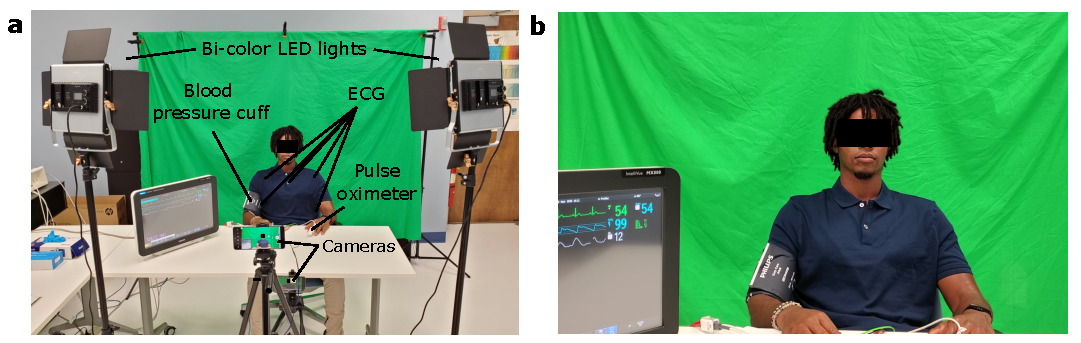
\includegraphics[width=\linewidth]{include/exp_setup_v2.pdf}
    \caption{\textbf{Constructing a diverse remote vital sign monitoring dataset with a focus on telemedicine applications.} (a) Experimental setup employed during the construction of the VITAL dataset. Two bi-color LEDs are used for controlled illumination of the subject, and laboratory tube LEDs are used for ambient illumination. The Philips IntelliVue MX800 patient monitor is utilized for ground truth vital sign monitoring. The subject wears a blood pressure cuff, 5-ECG leads, and a finger pulse oximeter, which is connected to the MX800 unit. Two smartphone cameras at differing viewing angles capture video of the subject. (b) Example frame from video captured by the front smartphone camera. Written consent was obtained from the subject for using their image in the publication.}
    \label{fig:exp_setup}
\end{figure}

To validate the performance of camera-based vital sign detectors, we construct the Vital-sign Imaging for Telemedicine AppLications (VITAL) dataset. The focus of this dataset is to represent diversity in factors that are relevant to telemedicine setups, including: (i) smartphone deployment, (ii) camera view angle, (iii) recording condition (lighting variation and talking), and (iv) patient demographic diversity. We address each of these aspects individually:

\begin{enumerate}[label=(\roman*)]
    \item \textbf{Smartphone deployment:} The ubiquity of smartphones globally has led to the development of patient portals, many of which can be accessed via smartphone applications that can be downloaded by patients \cite{mosa_systematic_2012,ventola_mobile_2014,boulos_how_2011}. Such applications have been used for hosting telemedicine appointments. A deployable remote HR estimation solution with a focus on telemedicine must be able to work efficiently on smartphone cameras by considering factors including video compression \cite{yu_remote_2019,nowara_systematic_2021,nowara_combating_2019} and algorithmic complexity. Moreover, the solution must achieve success independent of camera type. Hence, the VITAL dataset uses different smartphone cameras for each view angle. The use of more than one smartphone imager inspires the development of algorithms that can scale to a variety of device-agnostic telemedicine conditions. 
    \item \textbf{Camera view angle:} In a telemedicine setting, there can also be a variety of camera angles that the algorithm must work on. In order to facilitate this verification, the VITAL dataset consists of two camera view angles for all the videos of each subject (as seen in Figure~\ref{fig:exp_setup}).
    \item \textbf{Recording condition:} Another essential factor involves testing algorithms across a range of recording conditions, to promote the development of algorithms that can operate in the “wild”. The dataset consists of four recording conditions: (1) controlled lighting at 5600K (“cool” lighting) with the subject remaining stationary, (2) controlled lighting at 3200K (“warm” lighting) with the subject remaining stationary, (3) ambient room lighting- distributed white lighting- with the subject remaining stationary, and (4) ambient room lighting with the subject speaking. Additionally, a green screen backdrop is kept to potentially enable digital modification of background scenery.
    \item \textbf{Patient demographic diversity:} The VITAL dataset consists of 59 subjects spread across skin tone, age, gender, race, and ethnic backgrounds. Subject characteristics (gender, age, height, weight, body mass index, race, and ethnicity) are summarized in Table~\ref{tab:demographic} using mean (SD), median (IQR), or frequency (\%), unless otherwise noted. For the purpose of this study, we split the subjects into three skin tone categories based on the Fitzpatrick (FP) skin type scale \cite{fitzpatrick_validity_1988}: light, consisting of skin tones in the FP 1 and 2 scales, medium, consisting of skin tones in the FP 3 and 4 scales, and dark, consisting of skin tones in the FP 5 and 6 scales. This aggregation allows for more relevant trends, since any two consecutive FP scale categories are reasonably close.
\end{enumerate}

\begin{table}[]
\begin{center}
\scalebox{0.83}{
\begin{tabular}{lcl}
Total number of participants in study & \multicolumn{2}{c}{59} \\
 & \multicolumn{1}{l}{} &  \\
\textbf{Physical Demographics} & \multicolumn{1}{l}{\textbf{Mean}} & \textbf{Median} \\ \hline
Age (years) & 34 (10) & \multicolumn{1}{c}{34 (26-40)} \\
Height (cm) & 172 (10) & \multicolumn{1}{c}{174 (164-180)} \\
Weight (kg) & 73 (19) & \multicolumn{1}{c}{71 (57-82)} \\
Body Mass Index (kg m$^{-2}$) & 24 (7) & \multicolumn{1}{c}{24 (21-25)} \\
 & \multicolumn{1}{l}{} &  \\
\textbf{Sex} & \multicolumn{2}{l}{\textbf{\# of participants}} \\ \hline
Male & \multicolumn{2}{c}{36 (61\%)} \\
Female & \multicolumn{2}{c}{23 (39\%)} \\
 & \multicolumn{1}{l}{} &  \\
\textbf{Race} & \multicolumn{2}{l}{\textbf{\# of participants}} \\ \hline
White & \multicolumn{2}{c}{29 (49\%)} \\
Asian & \multicolumn{2}{c}{18 (31\%)} \\
Black or African American & \multicolumn{2}{c}{9 (15\%)} \\
Native Hawaiian or other Pacific Islander & \multicolumn{2}{c}{0 (0\%)} \\
American Indian or Alaska Native & \multicolumn{2}{c}{2 (3\%)} \\
Unknown & \multicolumn{2}{c}{1 (2\%)} \\
 & \multicolumn{1}{l}{} &  \\
\textbf{Ethnicity} & \multicolumn{2}{l}{\textbf{\# of participants}} \\ \hline
Hispanic/Latino & \multicolumn{2}{c}{7 (12\%)} \\
non-Hispanic/Latino & \multicolumn{2}{c}{52 (88\%)} \\
 & \multicolumn{1}{l}{} &  \\
\textbf{Skin Type} & \multicolumn{2}{l}{\textbf{\# of participants}} \\ \hline
Light & \multicolumn{2}{c}{21 (36\%)} \\
Medium & \multicolumn{2}{c}{26 (44\%)} \\
Dark & \multicolumn{2}{c}{12 (20\%)}
\end{tabular}} 
\end{center}

\caption{\textbf{Demographic characteristics of volunteers in the VITAL dataset.} Subject characteristics (gender, age, height, weight, body mass index, race, and ethnicity) are summarized using mean (SD), median (IQR), or frequency (\%).}
\label{tab:demographic}
\end{table}

The human study protocol was approved by the UCLA Institutional Review Board (IRB\#20-001025-AM-00001), and participants provided written informed consent to take part in the study. Figure~\ref{fig:exp_setup} shows the data collection setup. Each subject is made to sit on a height-adjustable chair, in the field of view of two cell-phone cameras (with different view angles): one camera (Samsung Galaxy S10) is perfectly front-on, while the other (Samsung Galaxy A51) is directly in front of the face, at a dip (lower) of 15 degrees. The front-on camera is placed approximately 130 cm from the subject, and the lower camera at a dip is approximately 90 cm from the subject. The height of the chair is chosen so that the subject is centered in the front-on frame. The controlled lights are set up on either side of the front-on camera, with a baseline of 100 centimeters between them.

As aforementioned, we record subjects using these cameras under four different scene conditions: (1) controlled lighting at 5600K (“cool” lighting) with the subject remaining stationary, (2) controlled lighting at 3200K (“warm” lighting) with the subject remaining stationary, (3) ambient room lighting (distributed white LED lighting) with the subject remaining stationary, and (4) ambient room lighting with the subject speaking. Controlled lighting is enabled by a pair of professional bi-color LED photography lights (Neewer Bi-Color 480 LED). The controlled lighting recording conditions were enabled with the room lights off, allowing for fine-tuned control over the illumination spectral properties. As incorporating controlled lighting only enables a front-facing illumination angle, two recording conditions in ambient room lighting were captured where the subject was lit more completely from several angles. The final recording condition involved variations in the subject, including talking, natural head movements, and facial expressions. Each scene recording session lasts for 2 minutes, for a total of 16 minutes of video footage across 8 videos. 

During data collection, volunteers are fitted with standard anesthesiology cardiopulmonary monitors: pulse oximeter (Red DCI, Masimo), blood pressure cuff (Comfort Care, Philips), and 5-lead electrocardiogram (Philips IntelliVue). To collect vital sign data, we utilize the Philips IntelliVue MX800 patient monitor to perform real time monitoring of four vital signs- HR, respiratory rate, oxygen saturation, and non-invasive continuous blood pressure- of which three waveforms are collected (ECG, PPG and respiration). We use the open source tool VSCapture \cite{karippacheril_data_2013} to collect data onto a computer using the MX800’s local area network communication protocol. The MX800’s estimated numeric values for the vital signs are sampled every 1 second, while the waveforms are sampled at variable frequencies. The ECG signal is sampled between 400-600 Hz, the PPG signal between 100-150Hz and the respiration between 40-60Hz.  Continuous non-invasive blood pressure estimates occur when the blood pressure cuff is activated, which is approximately once every 30 seconds. 

A total of 60 subjects participated in the study. Due to data collection errors, 1 subject is excluded from the experiment. Therefore, the final VITAL dataset consists of 472 videos ($\sim$944 minutes) of 59 subjects and their vital signs. The demographic characteristics of these volunteers is given in Table~\ref{tab:demographic}.

\section{The Diverse R-PPG pipeline}

\begin{figure}
    \centering
    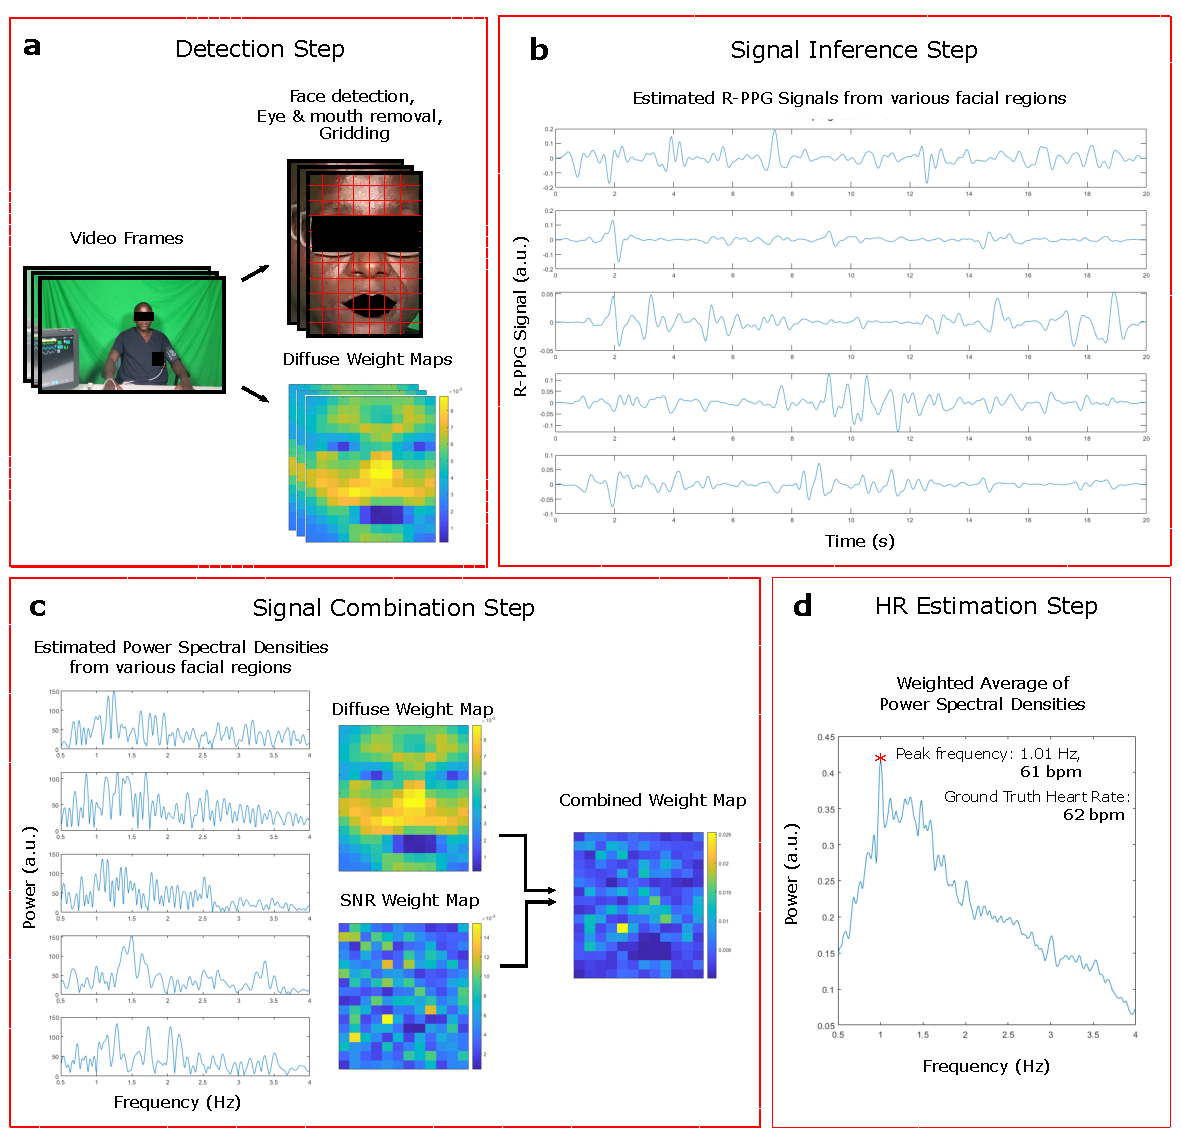
\includegraphics[width=0.75\linewidth]{include/fig6-pipeline.pdf}
    \caption{\textbf{The proposed contactless camera-based heart rate estimation algorithm consists of 4 steps.} The proposed novelty in the signal combination step of the pipeline incorporates skin diffuse information weighting, in addition to SNR weighting, to fuse signal information in the frequency-domain space in order to achieve robust R-PPG performance across skin tones. Written consent was obtained from the subject for using their image in the publication.}
    \label{fig:pipeline}
\end{figure}

There are four components to a typical R-PPG pipeline: (a) detection, which identifies facial regions of interest (ROI) in the video frame, (b) signal inference, which uses the RGB time series signals to estimate the pulsatile waveforms from the ROIs, (c) signal combination, which combines the information from the various estimated pulsatile waveforms, and (d) HR estimation, which estimates the HR from the combined information. 

From Section \ref{chap:theory}, we concluded that on top of other skin tone biases present in R-PPG algorithms and datasets, the main contributing factor to R-PPG skin tone bias is the fundamental light-transport bias that exists for subjects with a higher skin melanin fraction. Specifically, we showed that the R-PPG SNR drastically worsens with increasing skin melanin fraction, and therefore mitigating the skin tone bias present in R-PPG will require strategies that emphasize capturing more signal and reducing noise. As such, the primary innovation to the typical R-PPG pipeline will be in the signal combination step.  

The Diverse R-PPG pipeline is visually described in Figure~\ref{fig:pipeline}. The video is first passed through a neural network-based face detector \cite{zhang_joint_2016}, in order to identify the face region in the frame. Using feature point detectors \cite{kazemi_one_2014}, the eye and mouth regions are identified and explicitly removed from the videos (since these regions do not contribute to the pulsatile signal). Additionally, the diffuse component of the face is estimated using a specular highlight removal algorithm \cite{yang_real-time_2010}. Regions of interest are then obtained by dividing the facial frames into 192 grids of equal height and width. This is the detection step. The next steps, namely signal inference and signal combination and HR estimation, are carried out for smaller video-windows of 20 seconds length with an overlap of 10 seconds.

For signal inference, we choose the CHROM \cite{haan_robust_2013} signal extraction method due to its versatility and open availability of code \cite{mcduff_iphys_2019}. The spatially averaged RGB time series from each grid is used to estimate a pulsatile waveform. This waveform is then filtered using a 5th-order Butterworth bandpass filter with pass-band frequencies of [0.7, 4] Hz. These waveforms are used in the following signal combination step. 

In order to capture more signal and reduce noise, the pulsatile waveforms from the various ROIs on the face must be combined in a sensible manner. Traditionally, this combination does not occur after signal inference, but rather before when the pixels from the face are averaged for each frame. This is equivalent to defining only one grid or ROI, which is all the (skin-)pixels on the face. However, this naive averaging may not be optimal for noise reduction-- for example, regions on the face not corresponding to skin or containing large amounts of motion will contain noisy pulsatile information. 

To improve upon this, previous approaches have sought to modify this averaging process using a weighted average scheme. Most commonly, approaches have used a measure such as SNR at peak frequency of the estimated pulsatile waveform to characterize the `goodness' of each signal \cite{haan_robust_2013,po_block-based_2018,li_model-based_2020,kumar_distanceppg_2015,bobbia_unsupervised_2019}, and therefore be used as weights. The SNR can be estimated for a signal $s(t)$ (frequency domain $S(f)$) given a frequency $p$ that we suspect corresponds to the HR as follows:

\begin{equation}
    SNR=\frac{\int_{p-w}^{p+w}{\left|S(f)\right|^2df}+\int_{2(p-w)}^{2(p+w)}{\left|S(f)\right|^2df}}{\int_{-\infty}^{\infty}{\left|S(f)\right|^2df}-\int_{p-w}^{p+w}{\left|S(f)\right|^2df}-\int_{2(p-w)}^{2(p+w)}{\left|S(f)\right|^2df}}
\end{equation}

where $w$ is the peak window size for estimation (for this work’s experiments, we use $w=0.1$Hz). This essentially defines the signal power to be contained within a narrow-band of the fundamental and first harmonic of the HR frequency $p$, and regards the remaining signal power as noise.  

There are two major drawbacks to this method of signal combination. First, this method relies heavily on a good estimate of the initial HR frequency $p$. The $p$ used typically corresponds to the peak frequency of the signal from the naive facial aggregation method. As R-PPG is fundamentally biased with respect to skin tone, the estimate for $p$ is typically worse for darker skin tones. Moreover, the effect of noise more greatly affects darker skin tones. Consequently, it is empirically observed that the SNR weights for dark skin tones is far more variable window-to-window and sparse spatially. This means that this SNR weighting method of signal combination can actually worsen the skin-tone bias present in R-PPG (we observe this in our Results section). Second, this method of signal combination is done in the time-domain. However, it is not guaranteed that the pulsatile waveforms from different ROIs are aligned in time, either due to physical separation between the regions or due to the rolling-shutter of the video-camera. In other words, there may be a phase delay between the signals. The rolling-shutter effect is particularly relvant for R-PPG using smartphone cameras as highlighted by Mironenko \textit{et al.} \cite{mironenko_remote_2020}. 

To combat these issues, Diverse R-PPG makes two major novelities to the signal combination step: 
\begin{enumerate}[label=(\roman*)]
    \item \textbf{Combination in frequency-domain:} Ultimately, the goal is to estimate the HR of the subject. This relies on the frequency information contained within the estimated pulsatile waveform. The phase delay between estimated signals from different ROIs only affects the frequency content by a scalar constant. Therefore, by performing signal combination in the frequency-domain, namely through averaging the power spectral densities (PSD) of the inferred signals, sensible signal combination can be done without introducing additional artifacts. 
    \item \textbf{Novel weighting scheme:} From Section~\ref{sec:effect_noise_RPPG}, we concluded that specular reflections degrade the R-PPG signal. From the detection step, the estimated diffuse component can therefore be used as additional weights. The SNR weights from previous works and the novel diffuse weights are multiplied together and renormalized to arrive at the final weights used to combine the signals. The diffuse weights play two key roles: first, they can remove specular affected regions from the average explicitly. Second, they combat the sparsity issue observed in traditional SNR weights, since the diffuse component is continuous and non-sparse. 
\end{enumerate}

After computing the weighted average PSD using the novel weights and individual PSDs from the gridded pulsatile signals, the final HR is estimated by simply choosing the peak frequency. This summarizes the Diverse R-PPG pipeline for a single window. The pipeline can be iterated over multiple overlapping windows to estimate a beat-to-beat HR.  

\section{Benchmark methods and techniques}

To benchmark the performance of the proposed method, we compare the proposed method against previous R-PPG algorithms similar to our method. We compare with the two most common categories of signal combination steps that were described in the previous section, namely the naive pixel averaging, which we refer to as facial aggregation (c.f. \cite{poh_noncontact_2010,haan_robust_2013,wang_novel_2016,wang_algorithmic_2017,lewandowska_measuring_2011,de_haan_improved_2014}), and the modified SNR weighted averaging method, which we refer to as SNR weighting (c.f. \cite{po_block-based_2018,li_model-based_2020,kumar_distanceppg_2015,bobbia_unsupervised_2019}). 

To ensure a fair comparison with the benchmark methods, we implement identical testing conditions across techniques. For each method, the input video is passed through the same face detection algorithm (convolutional neural network-based detector \cite{zhang_joint_2016}), following which the eyes and mouth are cropped out using facial feature points \cite{kazemi_one_2014}. Some methods also use skin segmentation algorithms (\cite{wang_exploiting_2015,tang_noncontact_2018,villarroel_non-contact_2019}), but we empirically found this to perform slightly worse on the VITAL dataset. We also use a consistent HR selection technique for each method, namely the PSD is obtained using the amplitude of a fast Fourier transform and the HR is selected as the peak frequency.





